\chapter{Coding, Measurements and Limitations} % Measurements in next chapter? 
\label{chp:measurements}

The general idea of the sensor network is to collect data from the accelerometer,

\section{Nordic Semiconductor Example code}

Nordic Semiconductor has provided several examples along with the nRF52-DK documentation, that can be used as a starting point when programming applications to the device. 

\subsection{\gls{coap}}

As a first step, the nRF52 needed to communicate with the Raspberry Pi. As explained in section 2.6, a good starting point for this is to use the \gls{coap} trasnport protocol, and the example of the use of this on the device. The \textit{CoAP Server} and \textit{CoAP Observer} was loaded into two different nRF52 devices, and both of them connected to the Raspberry Pi. Now \gls{radvd} had to be activated on the Pi, to be able to use this as a \textit{forwarding server}. 

\begin{figure}[h]
    \centering
    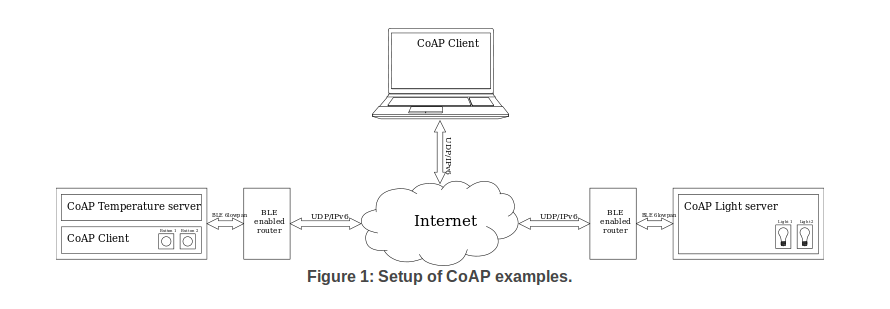
\includegraphics[scale=0.47]{CoAPExample.png}    
    \caption{CoAP Client-Server communication example}
    \label{fig:CoAPexample1}
\end{figure}

Figure \ref{fig:CoAPexample1} shows the initial CoAP example, by using two nRF52 devices, \gls{ble} over \gls{6lowpan} and a \gls{ble} enabled router (Raspberry Pi) on both ends in this case. As the figure \ref{fig:CoAPexample1} shows, the code example for the \gls{coap} client includes two different cases: 

\begin{itemize}
  \item In the fist case the \gls{coap} client acts as a client requesting services from the \gls{coap} server. Button 1 and 2 will control light 1 and 2 on the nRF52 server, which will send a conformation back if the light was changed or if something went wrong.
  \item In the second case the \gls{coap} server is excluded, but the \gls{coap} client works as a server that can handle requests from the router. In this case it is possible to use \textit{Copper} in a \textit{Firefox browser} on the Raspberry Pi to act as a client to request values from a simulated temperature sensor on the server. The server will  then send the current simulated temperature back, or tell if something went wrong. 
\end{itemize} 

When packets are captured using \textit{Wireshark}, we get the following capture: 

\begin{figure}[h]
    \centering
    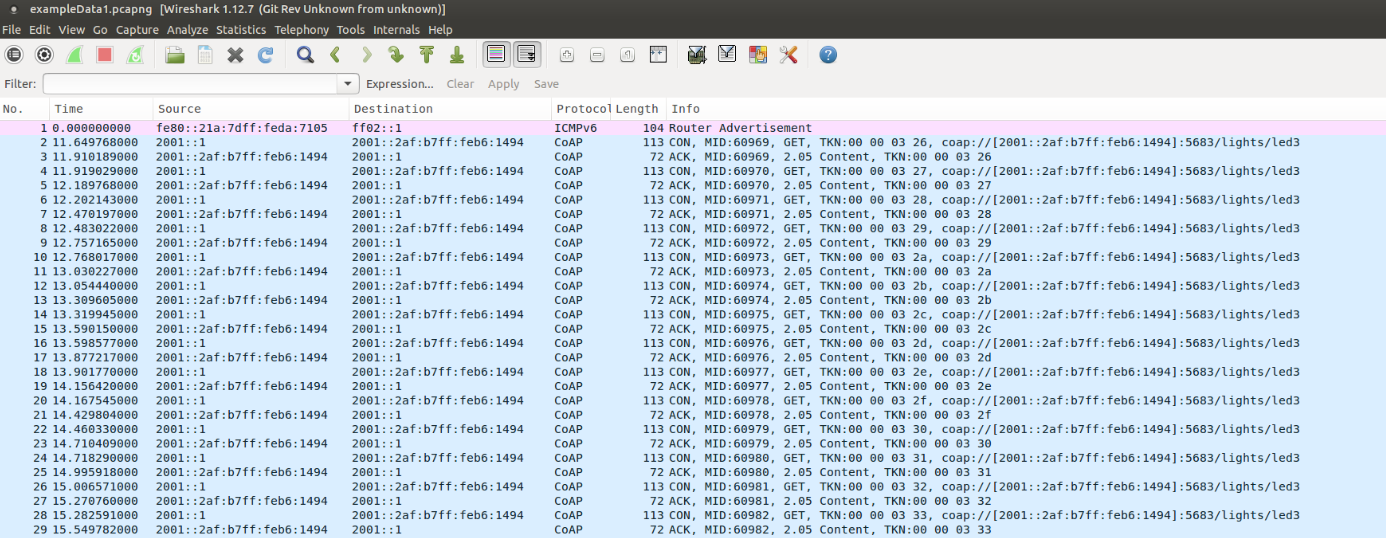
\includegraphics[scale=0.27]{CoapEx1captureCropped2.png}    
    \caption{CoAP Client-Server example Wireshark capture}
    \label{fig:CoAPexample1}
\end{figure}


This gives us the sequence diagram shown in Figure \ref{fig:seq1}. 

\begin{figure}[h]
    \centering
    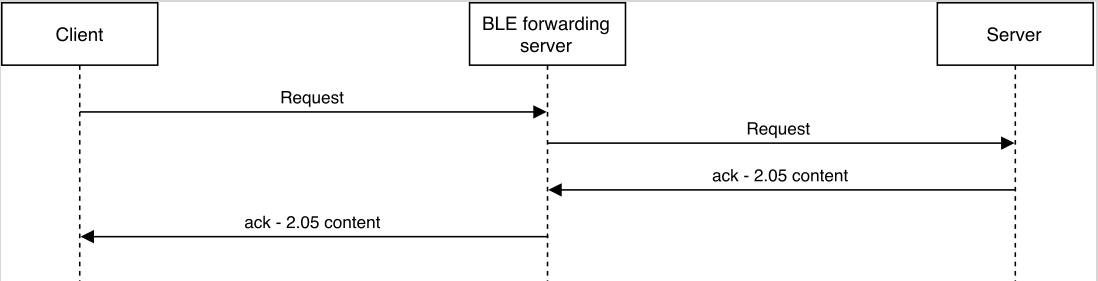
\includegraphics[scale=0.27]{seq1.png}    
    \caption{Sequence diagram CoAP Client-Server example}
    \label{fig:seq1}
\end{figure}

This works fine, but in the case of the system built in this thesis there is no need to receive a confirmation for every single message. The system is meant to be used with tools for analysing, and it is not essential that data needs to get to its destination right away. It therefore makes sense to send messages in an \textit{\gls{udp} fashion}, where packages are being sent right away without acknowledgement. This halves the number of packages sent, saves a lot of the network as well as actions needed to be done by the nRF52 where power consumption is a huge issue. Therefore the \textit{\gls{coap} Observable} function looked like an even better solution.   

\subsection{Observable \gls{coap}}

In the given Nordic example of a \gls{coap} observable server, this problem can be resolved. It is here easy to set up a server that can be observed by either a nRF52 client or a \gls{ble} forwarding server. The observable end point sends a \textit{CON-ACK request} in a given time interval to assure that the observing client is still there. As long as this message is being responded the server will continue to send data without any requirements of an \gls{ack}. 

\begin{figure}[h]
    \centering
    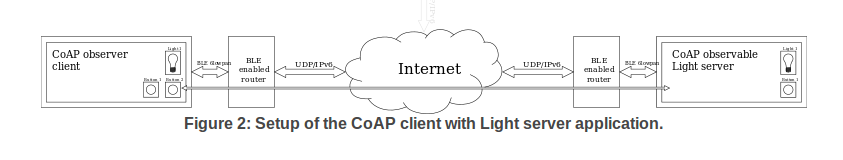
\includegraphics[scale=0.47]{CoAPObservalbFigure2.png}    
    \caption{CoAP Observable Server example}
    \label{fig:CoAPexample1}
\end{figure}

\section{Getting acceleration values}



\section{Bottle neck}

